
%(BEGIN_QUESTION)
% Copyright 2007, Tony R. Kuphaldt, released under the Creative Commons Attribution License (v 1.0)
% This means you may do almost anything with this work of mine, so long as you give me proper credit

Binary ``1'' and ``0'' states are not encoded using specific voltage levels in Ethernet systems as is the case with EIA/TIA-232, 422, or 485.  Rather, a different scheme known as {\it Manchester encoding} is used for Ethernet signals.  In Manchester encoding, each bit (either a 0 or a 1) is represented by a particular {\it transition} from low-to-high or from high-to-low.  In the IEEE standard for Manchester encoding, a high-to-low transition represents a ``0'' bit while a low-to-high transition represents a ``1'' bit.

Examine this Manchester-encoded signal on an oscilloscope screen, and determine the sequence of ``1'' and ``0'' bits represented by the waveform:

$$
\includegraphics[width=15.5cm]{i02203x01.eps}$$

\vskip 10pt

Hint: it may be easier to begin by sketching the waveform to represent a particular bit sequence.  For example, try sketching the Manchester encoded waveform to represent the bit sequence {\tt 1 0 1 1 0} first, then analyze the waveform given to you in this question.

\underbar{file i02203}
%(END_QUESTION)





%(BEGIN_ANSWER)

The data stream represented by the given waveform is {\tt 0 0 1 0 0}.

\vskip 10pt

Here is the waveform answer to the ``hint,'' where we encode the bitstream {\tt 1 0 1 1 0}:

$$
\includegraphics[width=15.5cm]{i02203x02.eps}$$

Note how one of the transitions does {\it not} represent a bit, but merely ``sets up'' the voltage level in preparation for another low-to-high (``1'') transition.  The key to deciphering a Manchester-encoded data stream is being able to identify which transitions represent real data bits and which do not.  Do you see the pattern, and how to distinguish one type of transition from the other?

\filbreak

Here's a clue to decoding a Manchester-encoded signal.  First, identify {\it all} signal transitions, as such:

$$\includegraphics[width=15.5cm]{i02203x04.eps}$$

Next, knowing that all {\bf data bits} are timed to a clock, and that these clock pulses are always equally spaced in time, you can see which transitions constitute data, and which are merely state reversals to set up the next bit.

$$\includegraphics[width=15.5cm]{i02203x03.eps}$$

\vskip 10pt

An advantage of Manchester encoding is that it encodes the clock signal directly into the data stream.  This helps devices synchronize each other without the need for a separate wire to carry a clock signal.  Auto-sensing 10/100 Mbit Ethernet hubs rely on this to tell what speed the incoming signals are going.

\vskip 10pt

A disadvantage of Manchester encoding is that the baud rate may be as high as twice the value of the bit rate.  For example, a Manchester-encoded 10 Mbps bitstream of all ones or all zeros would require a baud rate of 20 Mbaud, since each identical bit would require {\it two} voltage-level transitions.


%(END_ANSWER)





%(BEGIN_NOTES)


%INDEX% Electronics review: Manchester encoding
%INDEX% Networking, Ethernet: signal encoding

%(END_NOTES)


